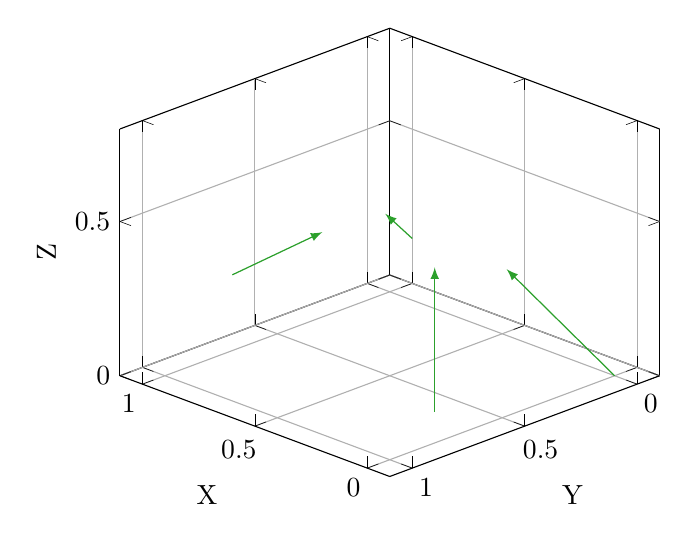
\begin{tikzpicture}

\definecolor{darkgray176}{RGB}{176,176,176}
\definecolor{forestgreen4416044}{RGB}{44,160,44}

\begin{axis}[
view={225}{30},
x grid style={darkgray176},
xlabel={X},
xmajorgrids,
xmin=-0.1, xmax=1.1,
xtick style={color=black},
y grid style={darkgray176},
ylabel={Y},
ymajorgrids,
ymin=-0.1, ymax=1.1,
ytick style={color=black},
z grid style={darkgray176},
zlabel={Z},
zmajorgrids,
zmin=0, zmax=0.8,
ztick style={color=black}
]
\addplot3 [draw=forestgreen4416044, line width=0.44pt, -latex, mark=none, quiver={u=\thisrow{u}, v=\thisrow{v}, w=\thisrow{w}}]
table [x=x,y=y,z=z] {%
x y z u v w
0 0 0 0.36 0.12 0.28
0.9 0 0.2 -0.16 0.28 0.2
0 0.8 0.1 0.2 -0.2 0.36
0.9 0.8 0.3 -0.24 -0.16 0.16
};
\end{axis}

\end{tikzpicture}
